\chapter{总体概述}

%Describes the general elements that may affect the product and the requirements on the product. It includes the following four parts. Note that this section should not describe the specific requirements, instead, it makes the specific requirements to be described more understandable.

%本节描述影响产品和产品需求的一般因素。由以下4个部分构成。 有一点需说明的是本节不描述具体的需求,只是使那些将要描述的具体需求更易于理解。
\section{软件概述}
\subsection{项目介绍}
% Describe the context and origin of the project being specified in this SRS. For example, state whether this project is a follow-on member of a project family, a replacement for certain existing systems, or a new, self-contained project.

% 描述本软件需求所描述的项目的背景。例如:本项目是一系列版本中的一个,或者是替代某个已经存在的系统,还是一个新的独立的项目。
本项目中将要实现的即时通讯系统,是一款跨平台、开源、可扩展的Web系统后端。通过Internet与各种平台上的客户端建立连接,来实现客户端之间多样化的消息传递。

\subsection{产品环境介绍}
% Describes the whole environment that is composed of this software and other products / projects.
% \begin{itemize}
% \item If this software is independent or fully self-contained, state it here.
% \begin{itemize}
% \item describe the function of each component of that larger system/project, and identify the interfaces.
% \item determine the main external interfaces of this software.( Note: Do not describe the interfaces in detail; the detailed description will be provided in other part of the SRS document.)
% \item describe related hardware of the product and peripheral equipment.( Note: This is only  a general description, not in detail.)
% \end{itemize}
% \end{itemize}

% It is very helpful to describe the main components, interconnection and external interfaces of the larger system/project by Block Diagram. This part should not provide a detailed design solution, or detailed design constraint for the solution (the detailed design constraint will be described in the section of specific requirement). This section is the basis of the design constraints.

% 描述的是本产品与其它产品或项目所组成的整体环境。

% 1.如果本产品是独立的并完全自我包含,在此说明这一点。

% 2.如果SRS定义的产品是更大的系统或项目的组件(此种情形经常发生),那么应:

% 	A. 描述此大系统或项目每个组件的功能,并且标识接口。

% 	B.  确定本软件产品主要外部接口。( 注意:在此部分并不进行这些接口的详细描述;对这些接口的详细描述在SRS的其它 部分提供。)
    
%   C. 描述相关产品硬件和所使用的外部设备。(  注意:  这只是概述性描述。)

% 通过方块图来描述大系统或项目的主要组件,互连性以及外部接口将是非常有帮助的。本部分不应提出一个具体的设计解决方案或对解决方案的具体设计约束(具体设计约束将在具体需求章节中描述)。本部分内容是产生设计约束的基础。
本项目的最终产品将分为服务端和客户端两大组件。
服务端为部署在服务器中的Web应用程序,运行在Linux或Windows Server平台上,为客户端提供服务。而整个聊天系统还包含:
客户端运行于Linux,Windows,Android,iOS等平台上,为用户提供操作接口。客户端可以是浏览器,也可以是定制开发的应用程序。
除此之外,整个系统所依赖的组件如下:
\begin{itemize}
	\item 服务器中使Web应用程序得以运行的代码解释器(如Python解释器)
	\item 服务器中使网络请求得以处理的网络中间件和服务程序(如Django框架和Apache Server)
\end{itemize}

\begin{figure}[h]
\centering
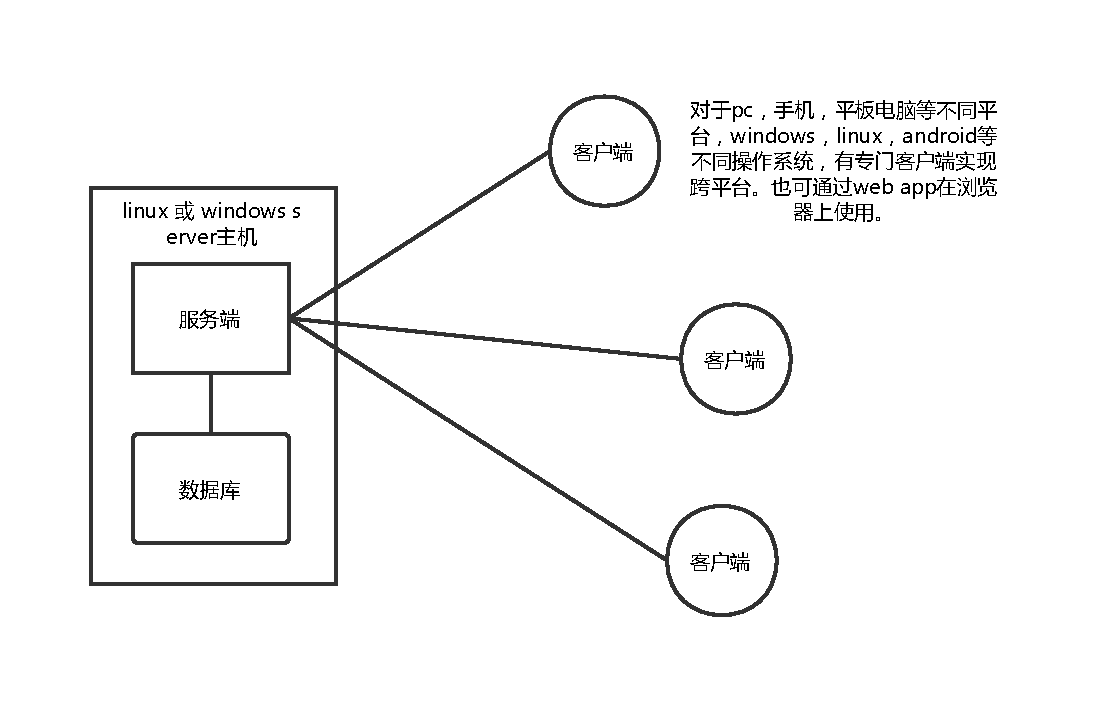
\includegraphics[width=13cm]{architecture}
\caption{系统架构} \label{fig:architecture}
\end{figure}

\section{软件功能}
% Summarizes the major functions that must be implemented through the software, and the functions to be implemented through user operation. Details will be provided in the Specific Requirement, so only a summary (such as a directory list) is needed here. The functions should be organized to make them understandable to the readers, and be appropriate for subsequent design and tests. Diagrams like top-level data flow diagram or object class diagram are recommended to illustrate the relationships among the major requirement groups 

% Sometimes, this section can directly refer to the superior specification of the software that allocate the specific requirements to this software ( if existed ).
% The specific requirements should not be described in this section. But this section is the basis of the specific requirements.

% 概述软件的必须实现的和通过用户操作实现的主要功能。这里只需要进行简要描述(例如目录列表),详细描述在详细需求部分描述。对需求功能进行组织,以便于读者理解,并能指导后续的设计和测试。可以用图表来表示主要需求群组之间的关系,例如:高层的数据流图,面向对象的分析等。

% 有时此部分所要求的功能概述可以从分配具体功能给此软件产品的更高层规格(如果存在的话)直接引用。

% 本节不应描述具体需求。但本节内容是具体需求章节的基础。
\begin{itemize}
	\item 注册,登录
	\item 一对一即时通讯
	\item 群聊
	\item 语音通话
	\item 视频通话
	\item 添加好友
	\item 表情包管理
	\end{itemize}

\section{用户特征}
%List down the basic required characteristics of the user or operator of the system. E.g. the experience, Skill level, required role etc., 
%This part should not describe the specific requirements, instead, it provides the basis for the specific requirements.
%
%列出对用户或系统操作者的要求,如:经验,能力,角色等。
%
%本节不应描述具体需求。但本节内容是具体需求章节的基础。

本系统分为服务端和客户端两大组件。

服务端的主要使用者为有搭建即时通讯系统需求的用户,要求具备一定的计算机知识和运维经验。

客户端的主要使用者为有即时通讯需求的用户,用户无需具备特殊的专业知识,但要求具有一定的计算机使用知识。

\section{假设和依赖关系}
% List any assumed factors (as opposed to known facts) that could affect the requirements stated in the SRS. These could include third party or commercial components that you plan to use, issues around the development or operating environment, or constraints. The project could be affected if these assumptions are incorrect, are not shared, or change. Also identify any dependencies the project has on external factors, such as software components that you intend to reuse from another project, unless they are already documented elsewhere (for example, in the vision and scope document or the project plan). 

% 列出可能影响SRS中需求的所有的假设因素(与已知事实相对而言),包括准备使用的第三方或商业组件,操作和开发环境的问题约束等。如果上述假设不正确、没有被告知或者改变了都将对项目产生影响。列出项目对外部条件的依赖,例如重用其他项目的模块等。如果在其他文档(例如项目计划或范围文档等)里已经描述了,在这里可以不用描述。
% 本文档所使用的假设条件包括:
\begin{itemize}
	\item 服务器端设备为x86体系结构
	\item 位于服务器的后端系统主要使用Python进行开发,而各个平台的客户端,均采用该平台专用的开发工具进行开发(如针对Android平台,使用Android Studio进行开发;针对Windows平台,使用Visual Studio进行开发)。
\end{itemize}